\chapter{State-of-the-Art} \label{chap:sota}

\section*{}

In this chapter we begin by making an in-depth presentation of essential concepts. This will be followed by a literature and state-of-the-art review in the fields of reverse engineering approaches that deal with Web applications, and approaches that infer patterns, in an effort to present state of the art and related work.

\section{Introduction}
In order to find the best approach to this problem, some research on already existing methodologies and concepts was needed. First an overview for the general categories researched is given, followed by the actual state of the art found, divided by relevant subcategories. 

\section{Concepts}

\subsection{Reverse Engineering}\label{sec:reverseengineering}

Reverse engineering is “the process of analyzing the subject system to identify the system components and interrelationships and to create representations of the system in another form or at a higher level of abstraction” \cite{chikofsky1990reverse}.

There are two types of reverse engineering: static and dynamic, depending on whether the model is extracted from the source code or from the program in execution, respectively \cite{systa1999dynamic}. Both approaches follow the same three main steps: \textit{collect} the data, \textit{analyse} it and \textit{represent} it in a legible way, and both allow obtaining information about control and data flow \cite{pacione2003comparative}.

\subsubsection{Static Analysis}

Static reverse engineering tries to extract information about an application through its source code or through its byte code. Static reverse engineering techniques may be useful during the development of a software system as a way of ensuring the correctness of the implementation or as a way of being aware of the current stage of the development \cite{systa2000static}.

A common technique useful for static analysis is code parsers based on grammars, as they are useful for code recognition. Apart from this, static analysis usually uses techniques of fact extraction, fact aggregation and querying \cite{telea2009querying, telea2008interactive}. 

\subsubsection{Dynamic Analysis}

Dynamic approaches extract information from the Application Under Analysis (AUA) in runtime, without access to the source code. Unlike the static techniques, dynamic approaches are able to extract information about concurrent behaviour, code coverage and memory management \cite{systa1999dynamic}.

\subsubsection{Other Methods}

Besides the previously mentioned methods, there is also the hybrid method, which combines static and dynamic analysis, and the historical method, which includes historic information to see the evolution of the software system \cite{canfora2011achievements}.

\subsection{Model-based Testing}

Model-based testing is the application of model-based design for designing, and optionally also executing artifacts to perform software testing or system testing. Models can be used to represent the desired behavior of a \textit{System Under Test} (SUT), or to represent testing strategies and a test environment. The process is illustrated in Figure \ref{fig:mbt}.

\begin{figure}[!htb]
\centering
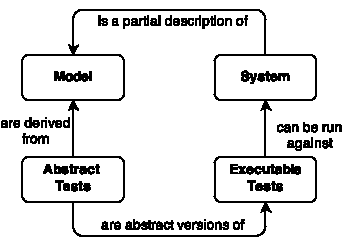
\includegraphics[width=0.6\textwidth]{mbt}
\caption{An explanation of the model-based testing process.}
\label{fig:mbt}
\end{figure}

A model describing a SUT is usually an abstract, partial presentation of the SUT's desired behavior. Test cases derived from such a model are functional tests on the same level of abstraction as the model. These test cases are collectively known as an \textit{abstract test suite}. An abstract test suite cannot be directly executed against an SUT because the suite is on the wrong level of abstraction, so an \textit{executable test suite} needs to be derived from a corresponding abstract test suite. 

The executable test suite can communicate directly with the system under test. This is achieved by mapping the abstract test cases to concrete test cases suitable for execution. In some model-based testing environments, models contain enough information to generate executable test suites directly; in others, elements in the abstract test suite must be mapped to specific statements or method calls in the software to create a concrete test suite. This is called solving the ``mapping problem" \cite{ammann2008introduction}. In the case of online testing, abstract test suites exist only conceptually but not as explicit artifacts.

Tests can be derived from models in different ways. Because testing is usually experimental and based on heuristics, there is no known single best approach for test derivation. It is common to consolidate all test derivation related parameters into a package that is often known as ``test requirements", ``test purpose" or even ``use case(s)" \cite{ammann2008introduction}. This package can contain information about those parts of a model that should be focused on, or the conditions for finishing testing (test stopping criteria).

Because test suites are derived from models and not from source code, model-based testing is usually seen as a form of \textit{black-box testing} (testing method in which the internal structure/design/implementation of the item being tested is not known to the tester).

\subsection{UI (User Interface) Patterns}
UI patterns (or \textit{interface design} patterns) are ways of capturing common structure without being too concrete on the details, which gives developers and interface designers the flexibility to be creative \cite{tidwell2010designing}. They are meant to be standard reference points, recurring solutions that solve common design problems. 

\section{Related Work}

\subsection{Extraction of Information from Execution Traces} \label{sec:extractexecutiontraces}

Plenty of approaches that extract information from execution traces have been found.\\
Elbaum \cite{elbaum2003improving} presents a testing approach that utilizes data captured in user sessions to create test cases. Duarte, Kramer and Uchitel defined an approach for behavior model extraction which combines static and dynamic information \cite{duarte2006model}. Sampath \textit{et al.} developed an approach for achieving scalable user-session-based testing of web applications, that applies concept analysis for clustering user sessions and a set of heuristics for test case selection \cite{sampath2007applying}. TraceServer \cite{andjelkovic2011trace} is an extension of the Java PathFinder model checking tool \cite{jpf} which collects and analyzes execution traces.  jRapture \cite{steven2000jrapture} is a technique and a tool for capture and replay of Java program executions. ReGUI \cite{coimbra2011reverse,coimbra2012dynamic} is a dynamic reverse engineering tool made to reduce the effort of modeling the structure and behavior of a software application GUI. Fischer \textit{et al.} developed a methodology that analyzes and compares execution traces of different versions of a software system to provide insights into its evolution, named EvoTrace \cite{fischer2005system}. Amalfitano's approach \cite{amalfitano2010rich} generates test cases from execution traces to help testing from Rich Internet Applications (RIAs), with the execution traces being obtained from user sessions and crawling the application. 

\subsection{Extraction of Information from Applications}

The following approaches extract information from Web, desktop and mobile applications for analysis, processing and testing.\\
Ricca and Tonella's ReWeb \cite{ricca2001understanding} dynamically extracts information from a Web application's server logs to analyze its structure and evolution, and so aims to find inconsistencies and connectivity problems.
Benedikt \textit{et al.} introduced a framework called VeriWeb \cite{benedikt2002veriWeb} that discovers and explores automatically Web-site execution paths that can be followed by a user in a Web application.
Di Lucca \textit{et al.}'s approach \cite{di2005integrating} integrates WARE \cite{di2004reverse}, a static analysis tool that generates UML diagrams from a Web application's source code, and WANDA \cite{antoniol2004understanding}, a Web application dynamic analysis tool, to identify groups of equivalent built client pages and to enable a better understanding of the application under study.
Bernardi \textit{et al.} \cite{bernardi2008reverse} presents an approach for the semi-automatic recovery of user-centered conceptual models from existing web aplications, where the models represents the application's contents, their organization and associations, from a user-centered perspective.
Marchetto \textit{et al.} proposed a state-based Web testing approach \cite{marchetto2008state} that abstracts the Document Object Model (DOM) into a state model, and from the model derives test cases.
Crawljax \cite{roest2010automated} is a tool that obtains graphical site maps by automatically crawling through a Web application.
WebDiff \cite{choudhary2010Webdiff} is a tool that searches for cross-browser inconsistencies by analyzing a website's DOM and comparing screenshots obtained in different browsers.
Memon presented an end-to-end model-based Web application automated testing approach \cite{memon2007event} by consolidating previous model development work into one general event-flow model, and employs three ESESs (event space exploration strategies) for model checking, test-case generation, and test-oracle creation.
Mesbah \textit{et al.} proposed an automated technique for generating test cases with invariants from models inferred through dynamic crawling \cite{mesbah2012invariant}. Another approach by Mesbah \textit{et al.}, named FeedEx \cite{fard2013feedback} is a feedback-directed Web application exploration technique to derive test models. It uses a greedy algorithm to partially crawl a RIA's GUI, and the goal is that the derived test model capture different aspects of the given Web application's client-side functionality. 
Artzi \textit{et al.} developed a tool called Artemis \cite{artzi2011framework} which performs feedback-directed random test case generation for Javascript Web applications. Artemis triggers events at random, but the events are prioritized by less covered branch coverage in previous sequences.
Amalfitano \textit{et al.} developed a semi-automatic approach \cite{amalfitano2011using} that uses dynamic analysis of a Web application to generate end user documentation, compliant with known standards and guidelines for software user documentation.
Dincturk \textit{et al.} \cite{dincturk2012statistical} proposed a RIA crawling strategy using a statistical model based on the model-based crawling approach introduced in \cite{benjamin2011strategy} to crawl RIAs efficiently.
Dallmeier \textit{et al.}'s Webmate \cite{dallmeier2012Webmate,dallmeier2013Webmate} is a tool that analyzes the Web application under test, identifies all functionally different states, and is then able to navigate to each of these states at the user’s request.
Amalfitano \textit{et al.}'s approach, AndroidRipper \cite{amalfitano2012using}, uses ripping to automatically and systematically traverse the app’s user interface, generating and executing test cases as new events are encountered.

\subsection{Model Extraction from Applications via Reverse Engineering}

There are plenty of approaches that extract models from desktop and Web applications, even if the extracted models may be different from the models extracted by this application. Memon's GUI Ripping \cite{memon2003gui} is an approach that reverse engineers a model represented as structures called a GUI forest, event-flowgraphs and an integration tree directly from the executable GUI. Paiva \textit{et al.}'s approach \cite{paiva2007towards,paiva2008reverse} reverse engineers structural and behavioural formal models of a GUI application by a dynamic technique, mixing manual and automatic exploration with the goal of diminishing the effort required to construct the model required in a model-based GUI testing process. Sanchez \textit{et al.}'s approach \cite{sanchez2010model} is a model-driven engineering process that performs reverse engineering of the layout of RAD-built GUIs, and produces a GUI model in order to perform actions like adapt the GUI for mobile device screens. Gimblett and Thimbleby's approach \cite{gimblett2010user} discovers automatically a model of an interactive system by exploring the system's state space, and uses the produced models for structural usability analysis. Scheetz \textit{et al.} have used a class diagram representation of the system’s architecture to generate test cases using an AI planning system \cite{scheetz1999generating}. Moore \cite{moore1996rule} describes experiences with manual reverse engineering of legacy applications to build a model of the user interface functionality. Silva \textit{et al.}'s GUISurfer \cite{Silva:2010:GTT:1822018.1822045} is a framework that extracts behavioural models from the source code of GUI-based applications, in order to test their implementation. Lutteroth's approach \cite{Lutteroth:2008:ARE:1378337.1378350} is able to recover a higher-level layout representation of a hardcoded GUI using the Auckland Layout Model \cite{Zeidler:2013:ALE:2501988.2502007}. Belluci \textit{et al.}'s approach \cite{Bellucci:2012:ARE:2166966.2167004} performs reverse engineering of interactive dynamic Web applications into a model-based framework able to describe them at various abstraction levels, with the goal of facilitating the adaptation of the analysed Web applications to other types of interactive devices. Stojanovic \textit{et al.}'s approach \cite{stojanovic2002reverse} is a semi-automated reverse engineering approach to generate shared-understandable metadata of Web applications, in order to migrate the applications to the Semantic Web.

\subsection{Inferring Patterns from Web applications}

Despite the fact that there are plenty of approaches to mine patterns from Web applications, no approaches have been found that infer UI patterns from Web applications beside the work this dissertation means to extend \cite{nabuco2013inferring, morgado2012gui}. The approaches found deal mostly with Web mining, with the goal of finding relationships between different data or finding the same data in different formats. Brin \cite{brin1999extracting} presented an approach to extract relations and patterns for the same data spread through many different formats. Chang \cite{chang2003automatic} proposes a similar method to discover patterns, by extracting structured data from semi-structured Web documents. Freitag \cite{freitag1998information} proposed a general-purpose relational learner for information extraction from Web applications.

\section{UI Patterns}\label{sec:patterns}

User Interaction (UI) patterns are well-documented in a various number of sources \cite{tidwell2010designing, van2001patterns, neil12standard, sinnig2005patterns}. The patterns already supported (like the Search and Master/Detail patterns) enter the list of most popular patterns, according to the sources found, and if the selection of supported patterns were to be broadened, the pick of the next one(s) would be heavily influenced by the literature. Lin and Landay's approach \cite{lin2008employing} uses UI patterns for Web applications that run on PCs and mobile phones, and prompt-and-response style voice interfaces. Pontico \textit{et al.}'s approach \cite{pontico2008organizing} presents UI patterns common in eGovernment applications. In \cite{4bestlibs} are presented the four best user interface pattern libraries, chosen by the UX Movement community.

\subsection{Capture-Replay Tools}

The execution traces of a Web application, on the client side, are usually captured via a capture-replay tool. Here we present the most popular capture-replay tools used nowadays.

Selenium \footnote{Selenium: \url{http://docs.seleniumhq.org/}} is an open-source capture/replay tool that captures an user's interaction with a Web application in HTML files. It has multi browser, OS and language support, can be installed server-side and as a Mozilla Firefox add-on, has its own IDE \textit{(Integrated Development Environment)}, and allows recording and playback of tests.

Watir Webdriver \footnote{Watir: \url{http://watirwebdriver.com/}} is is an open-source (BSD) family of Ruby libraries for automating Web browsers and Web application testing. It has multi browser and OS support, a rich API, and has a functionality for non-tech users: the ‘Simple’ class. There also exist ports for other programming languages, such as \textit{Watij} (for Java) and \textit{Watin} (.NET).

IBM Rational Functional Tester (RFT) \footnote{IBM RFT: \url{http://www-03.ibm.com/software/products/en/functional}} is an automated functional testing and regression testing tool. This software provides automated testing capabilities for functional, regression, GUI, and data-driven testing. Rational Function Tester supports a range of applications, such as .Net, Java, Siebel, SAP, terminal emulator-based applications, PowerBuilder, Ajax, Adobe Flex, and others. It permits storyboard testing, automated testing, data-driven testing, and test scripting.

Sahi \footnote{Sahi: \url{http://sahi.co.in/}} is an open-source automation and testing tool for web applications. It allows recording and replaying across browsers, provides different language drivers for writing test scripts, and supports Ajax and highly dynamic web applications. 

\section{Chapter Conclusions}

In this chapter we gave a brief introduction of the concepts that serve as base to the thesis. We also presented related works on the areas of reverse engineering approaches that extract information from applications in general and Web applications in specific, approaches that extract models automatically from applications, and approaches that infer patterns from applications. Lastly, we presented documentation on UI patterns, and presented various capture/replay applications.

Most of the presented approaches that extract information from execution traces consume execution traces with different content than the ones the developed tool uses; the execution traces range from server logs, to sequences of actions enriched with context information like system state, to sequences of executed code instructions in a run path. Similarly, the presented approaches that extract general information from applications do so for many purposes: for testing (and in this category we test generation, model checking, and use case derivation), analysis, to search for inconsistencies, to better understand a Web application, to generate documentation, and others. 

The applications that more closely ressemble the developed approach are the ones that extract models from Web applications, and in that category, the extracted models vary in content. Some extract the layout of the Web application; others extract a directed finite graph, which represents the states of the applications and the actions necessary to switch between states; and some use logical database models. Few model extraction approaches extract models from the GUI of the Web application, and those that do, do so for user interface reengineering (typically of legacy systems).

Finally, there have not been found approaches that extract UI patterns from applications. There are approaches that infer patterns, but the inferrable patterns are other types of patterns: design patterns, textual patterns from databases (related to the field of knowledge and text mining), or Web mining. Additionally, there are few, if none, approaches that mine patterns from GUIs. The closest we've found was an approach that mined usage patterns (common action sequences executed by users) from Web applications, which relates more to Web mining than model extraction.